\section{Results}

\subsection{Multi-Seed Performance}

Table~\ref{tab:multiseed} summarizes the performance of the four experimental scenarios over five random seeds. The CNN with texture fusion (E2) obtained the highest average performance, with a macro-F1 of $0.9993 \pm 0.0015$ and an accuracy of $0.9993 \pm 0.0015$. The segmentation-only model (E1) achieved a macro-F1 of $0.9976 \pm 0.0029$, while the proposed segmentation-texture hybrid model (E3) achieved a similar macro-F1 of $0.9976 \pm 0.0035$. The baseline CNN (E0) obtained the lowest average macro-F1, with $0.9969 \pm 0.0052$.

Although all models achieved high classification performance, the results show different trade-offs. E2 obtained the best average macro-F1, but it required more parameters and a larger model size than E0 and E1. E1 achieved the lowest average inference time, with $2.7714 \pm 0.4108$ ms/image, while maintaining high predictive performance. E3 remained competitive, but it did not outperform E2 in average macro-F1 and had a larger model size than the non-texture CNN variants.

\begin{table*}[t]
\caption{Multi-seed summary over five runs. Values are reported as mean $\pm$ standard deviation.}
\label{tab:multiseed}
\centering
\footnotesize
\begin{adjustbox}{width=\textwidth}
\begin{tabular}{lccccccc}
\toprule
Model & Accuracy & Macro-Precision & Macro-Recall & Macro-F1 & Inference (ms/img) & Parameters & Size (MB) \\
\midrule
E0 Baseline CNN &
$0.9969 \pm 0.0053$ &
$0.9970 \pm 0.0052$ &
$0.9969 \pm 0.0053$ &
$0.9969 \pm 0.0052$ &
$3.9542 \pm 0.7074$ &
2.23M &
8.74 \\

E1 Segmented CNN &
$0.9975 \pm 0.0030$ &
$0.9977 \pm 0.0027$ &
$0.9975 \pm 0.0030$ &
$0.9976 \pm 0.0029$ &
$2.7714 \pm 0.4108$ &
2.23M &
8.74 \\

E2 CNN + Texture &
$\mathbf{0.9993 \pm 0.0015}$ &
$\mathbf{0.9994 \pm 0.0014}$ &
$\mathbf{0.9993 \pm 0.0015}$ &
$\mathbf{0.9993 \pm 0.0015}$ &
$4.3820 \pm 0.7072$ &
2.59M &
10.12 \\

E3 Segmented CNN + Texture &
$0.9975 \pm 0.0036$ &
$0.9977 \pm 0.0033$ &
$0.9975 \pm 0.0037$ &
$0.9976 \pm 0.0035$ &
$3.5657 \pm 0.7854$ &
2.59M &
10.12 \\
\bottomrule
\end{tabular}
\end{adjustbox}
\end{table*}

\subsection{Statistical Comparison Against the Baseline}

To evaluate whether the enhanced configurations produced consistent improvements over the baseline, paired macro-F1 differences were computed against E0 using the same five seeds. Table~\ref{tab:statistical_comparison} reports the mean macro-F1 deltas and Wilcoxon signed-rank test results.

E2 obtained the largest average improvement over E0, with a mean macro-F1 delta of $+0.0024$. E1 and E3 also showed positive average deltas, with $+0.0007$ and $+0.0007$, respectively. However, the Wilcoxon signed-rank test did not indicate statistically significant differences for any enhanced scenario. The obtained $p$-values were 1.00 for E1 versus E0, 0.75 for E2 versus E0, and 1.00 for E3 versus E0. Therefore, although the enhanced variants improved the average macro-F1, these differences were not statistically significant under the five-seed evaluation.

\begin{table}[t]
\caption{Paired macro-F1 comparison against the baseline.}
\label{tab:statistical_comparison}
\centering
\footnotesize
\setlength{\tabcolsep}{4pt}
\begin{tabular}{lccc}
\toprule
Comparison & $\Delta$ Macro-F1 & Std. & $p$-value \\
\midrule
E1 -- E0 & $+0.0007$ & 0.0069 & 1.00 \\
E2 -- E0 & $+0.0024$ & 0.0059 & 0.75 \\
E3 -- E0 & $+0.0007$ & 0.0057 & 1.00 \\
\bottomrule
\end{tabular}
\end{table}

\subsection{Aggregate Confusion Matrix Analysis}

To complement the metric-based evaluation, confusion matrices were aggregated across the five seeds for each model. Since each seed was evaluated on 891 test images, each aggregate confusion matrix summarizes 4,455 predictions per experimental scenario.

The aggregate results confirm the trend observed in Table~\ref{tab:multiseed}. The baseline model (E0) produced 4,441 correct predictions and 14 errors, corresponding to an aggregate accuracy of 0.9969. The texture-fusion model (E2) produced 4,452 correct predictions and only 3 errors, corresponding to the highest aggregate accuracy of 0.9993. The proposed hybrid model (E3) produced 4,444 correct predictions and 11 errors, corresponding to an aggregate accuracy of 0.9975. Therefore, E3 improved over the baseline in aggregate accuracy, but E2 remained the strongest configuration overall.

Figure~\ref{fig:aggregate_confusion_matrices} compares the aggregate confusion matrices for E0, E2, and E3. E0 is included as the baseline reference, E2 is included because it obtained the highest average macro-F1 and the lowest number of aggregate errors, and E3 is included because it corresponds to the proposed segmentation-texture hybrid architecture. The aggregate matrices show that most errors occurred among visually similar disease classes, while Tungro remained highly stable across the evaluated configurations.

\begin{figure*}[t]
\centering
\begin{minipage}{0.32\textwidth}
\centering
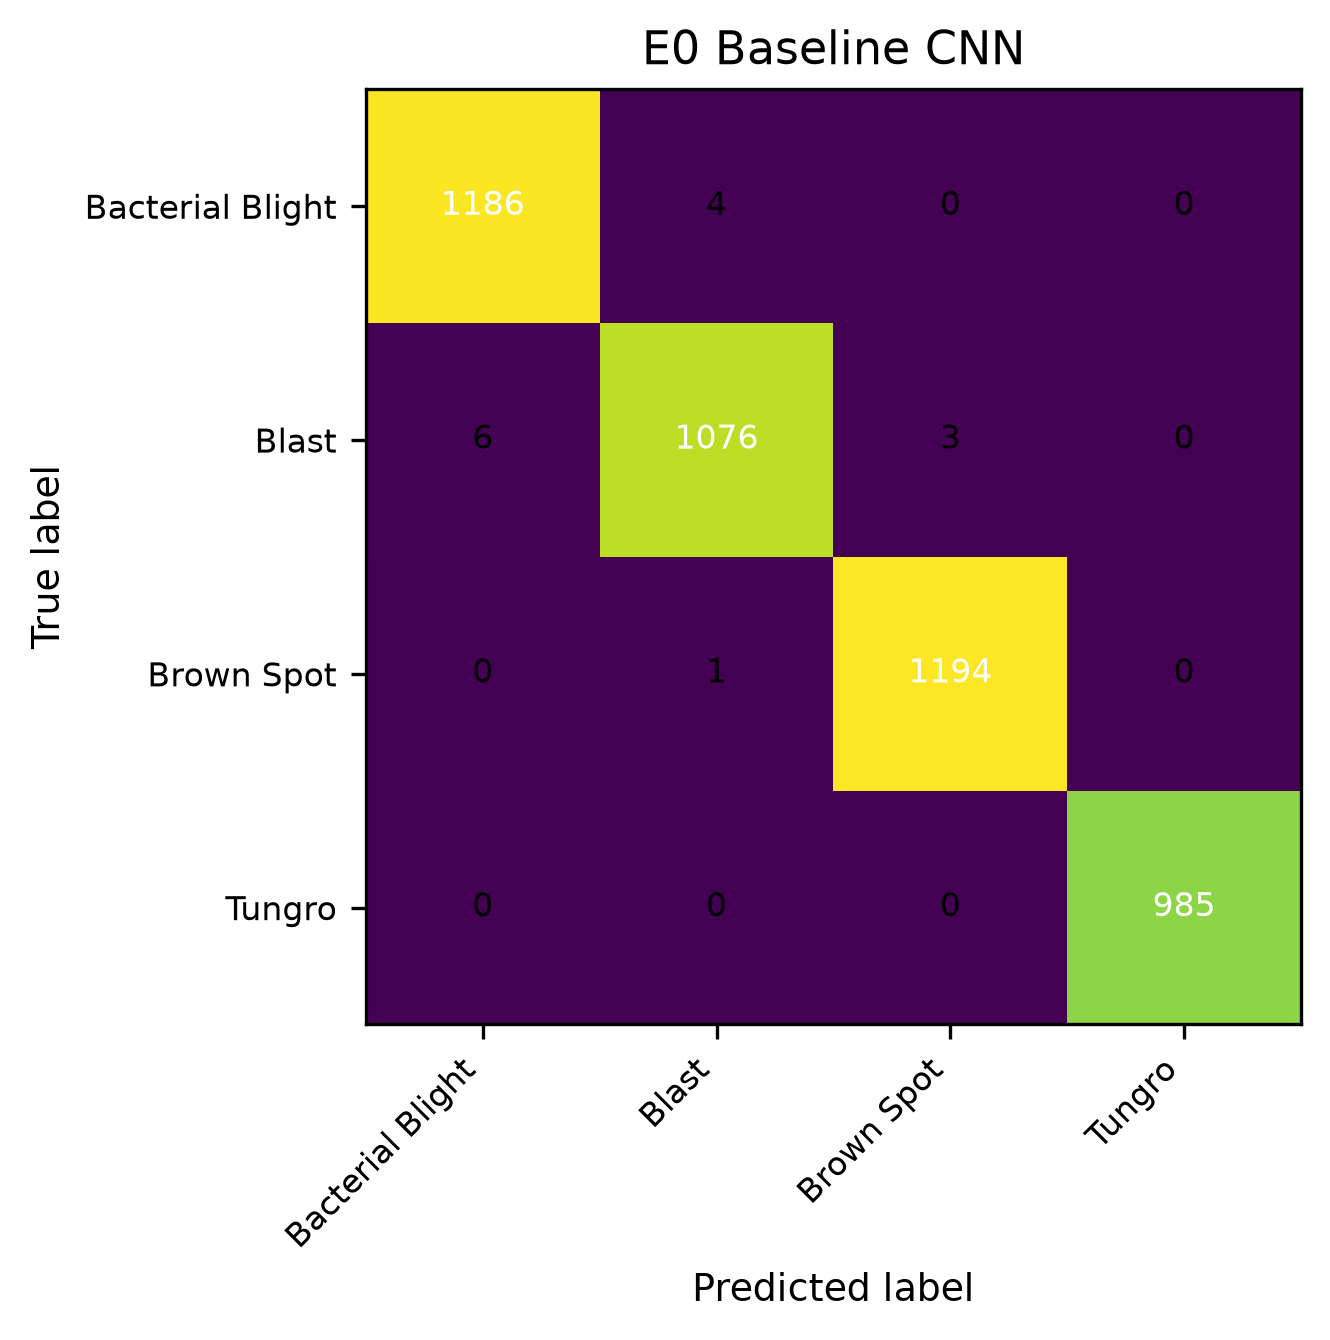
\includegraphics[width=\linewidth]{figures/fig03_aggregate_confusion_e0.png}
\centerline{(a) E0 baseline CNN}
\end{minipage}
\hfill
\begin{minipage}{0.32\textwidth}
\centering
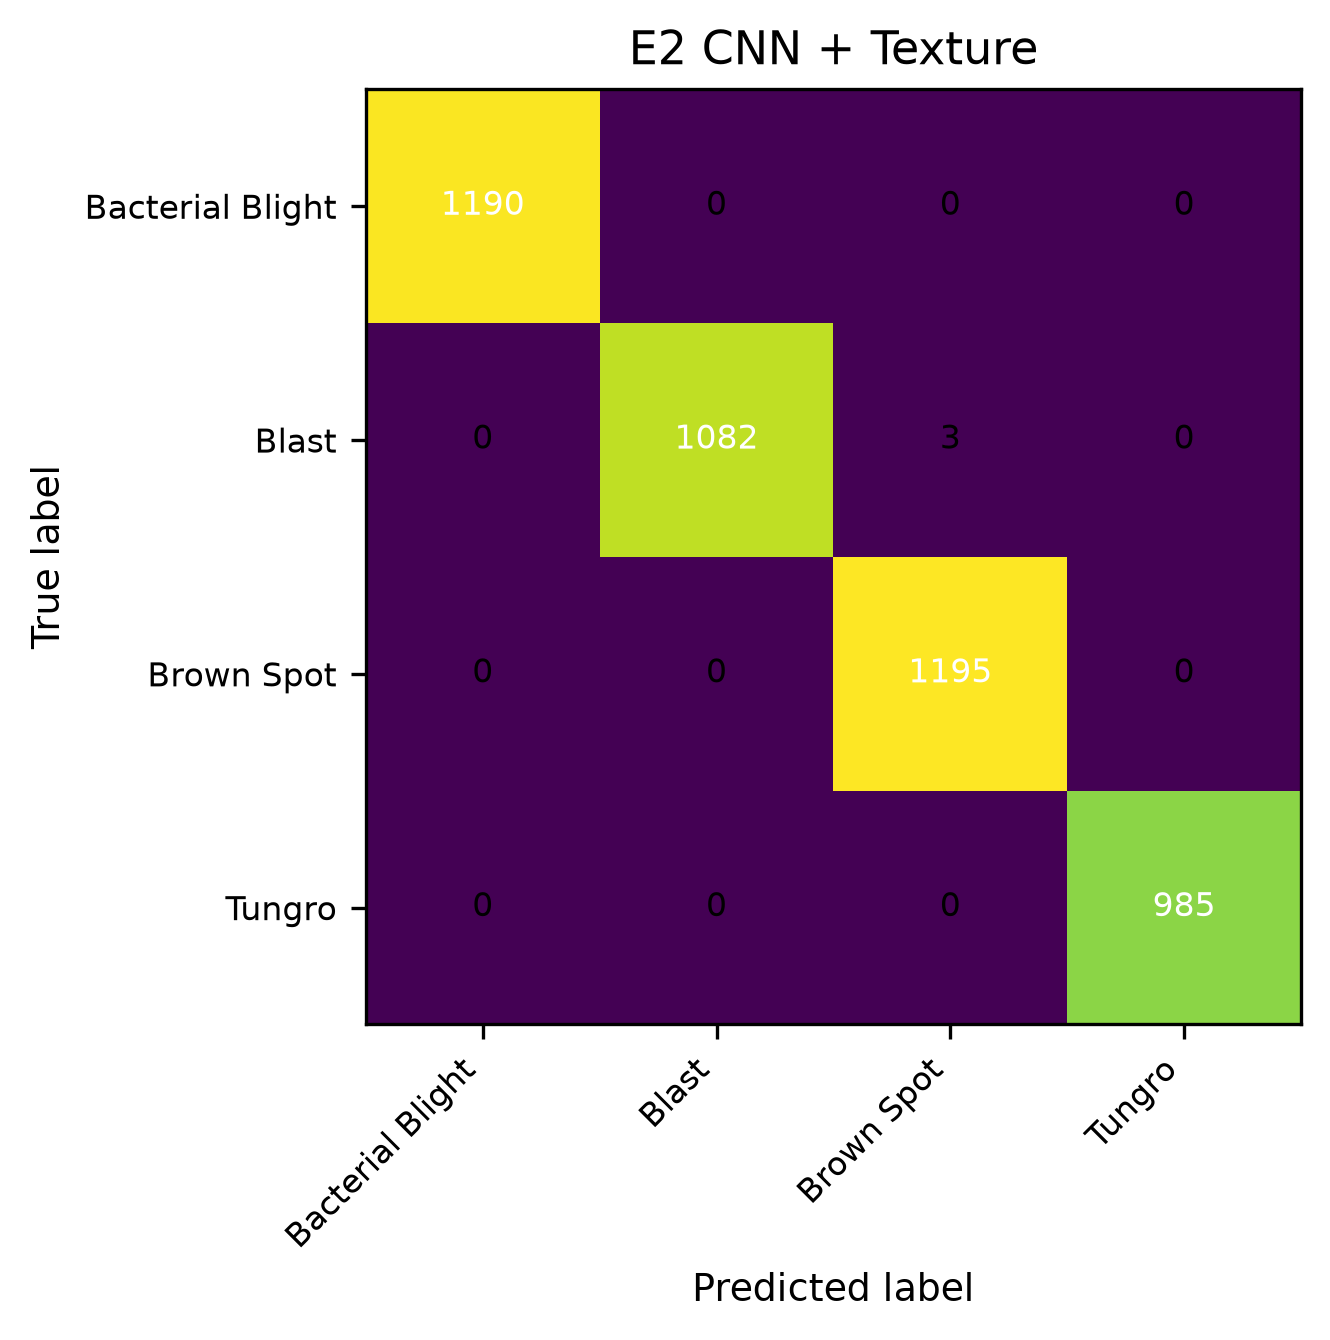
\includegraphics[width=\linewidth]{figures/fig04_aggregate_confusion_e2.png}
\centerline{(b) E2 CNN + texture}
\end{minipage}
\hfill
\begin{minipage}{0.32\textwidth}
\centering
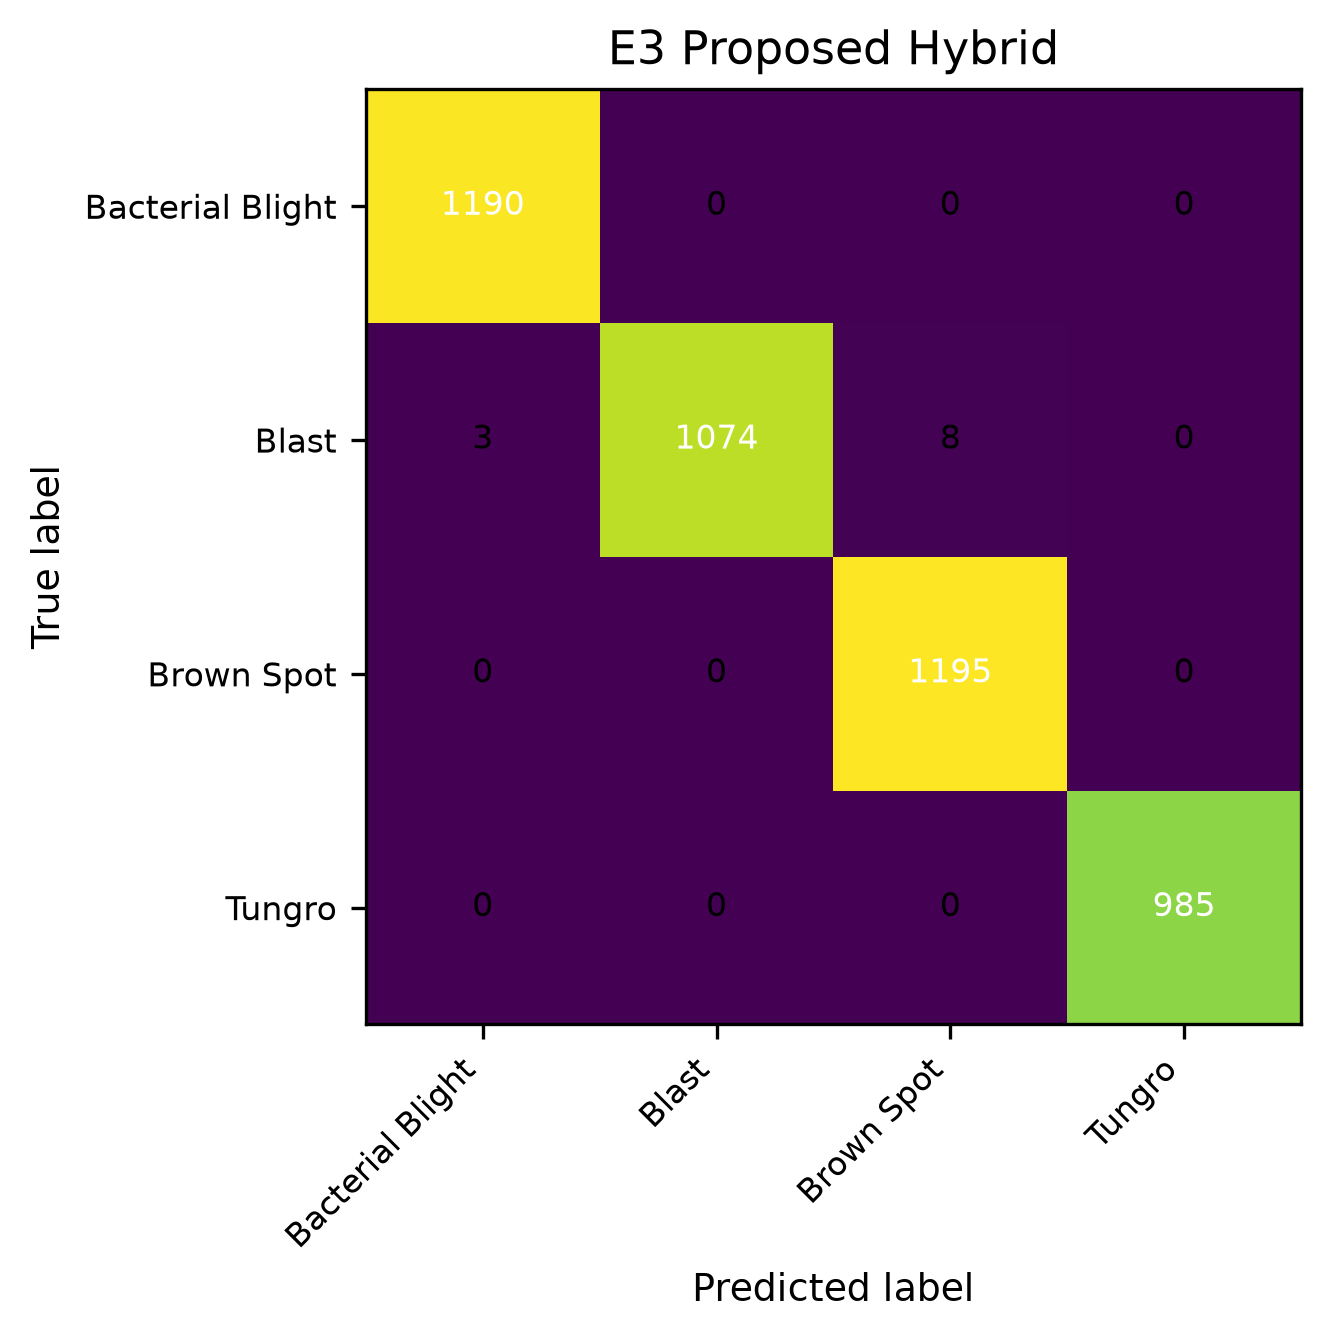
\includegraphics[width=\linewidth]{figures/fig05_aggregate_confusion_e3.png}
\centerline{(c) E3 proposed hybrid}
\end{minipage}
\caption{Aggregate confusion matrices over five seeds. Each matrix summarizes 4,455 predictions. E0 is shown as the baseline, E2 as the best average model, and E3 as the proposed segmentation-texture hybrid model.}
\label{fig:aggregate_confusion_matrices}
\end{figure*}
